\documentclass[12pt,a4paper]{article}
\usepackage[utf8]{inputenc}
\usepackage[spanish]{babel}
\usepackage{float}
\usepackage{amsmath}
\usepackage{amsfonts}
\usepackage{subcaption}
\usepackage{amssymb}
\usepackage{graphicx}
\usepackage{hyperref}
\graphicspath{{Pics/}}
\title{Caminatas Cuánticas en 4D}
\author{}
\date{}

\begin{document}

\maketitle

\tableofcontents
\newpage

\section{Matemática}
Pendiente.

\section{El estado del caminante para tiempos largos}

Se tiene la intuición de que la geometría del estadio es el único factor que juega un papel en la emergencia del caos cuántico. Siguiendo la motivación de un contexto clásico, se sabe que la partícula libre en un estadio rectangular es integrable, mientras que, si la partícula está confinada en un estadio del tipo Bunimovich, se observa caos clásico (coeficiente de Lyapunov positivo). 

Las siguientes figuras muestran cómo se ve la distribución de probabilidad espacial del caminante para ciertos tiempos en su evolución: 

\begin{figure}[H]
    \centering
    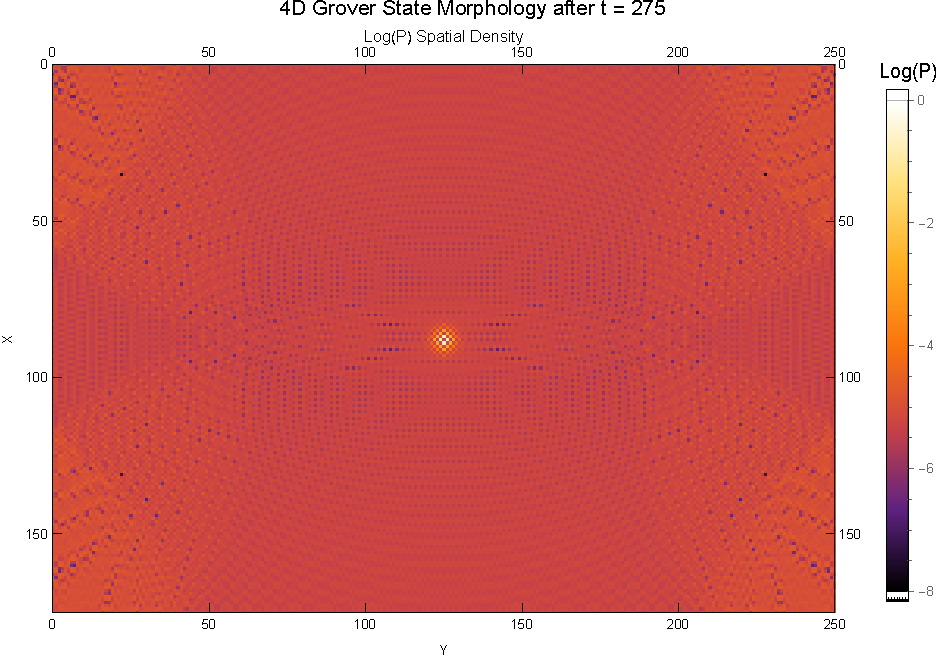
\includegraphics[width=0.8\textwidth]{RectangleStateTimeEvol.pdf}
    \caption{Evolución de un estado localizado con estado inicial de moneda $(1,1,1,1)$ en el tiempo $t=275$ pasos. Dimensiones del estadio: $L_x=200$, $L_y=175$. Moneda de Grover: $\pi/4$.}
\end{figure}
\begin{figure}[H]
    \centering
    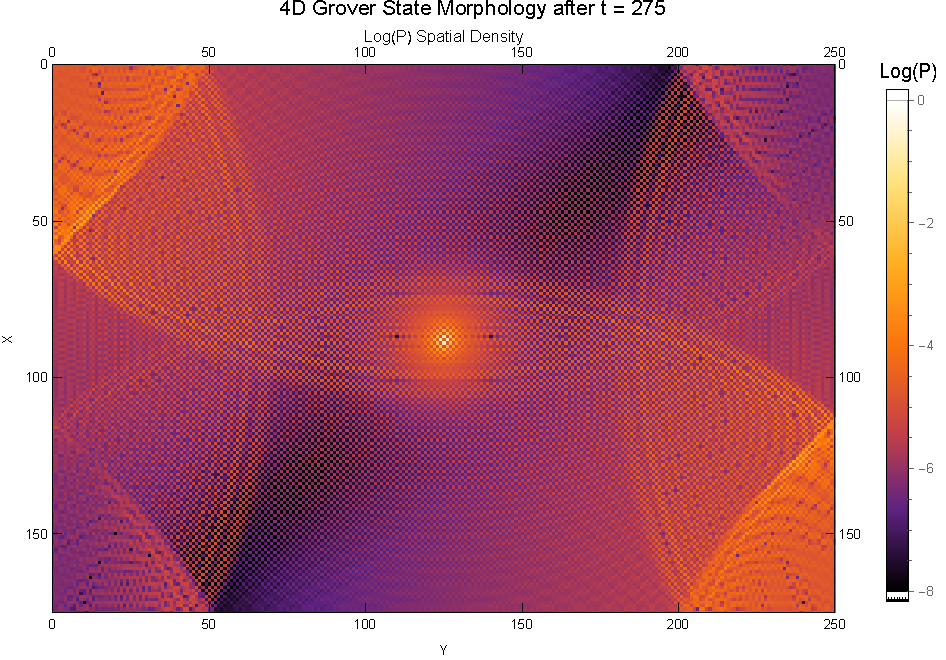
\includegraphics[width=0.8\textwidth]{RectangleStateTimeEvolNonSymCoin.pdf}
    \caption{Evolución de un estado localizado con estado inicial de moneda $(1,-1,1,-1)$ en el tiempo $t=275$ pasos. Dimensiones del estadio: $L_x=200$, $L_y=175$. Moneda de Grover: $\pi/4$.}
\end{figure}
\begin{figure}[H]
    \centering
    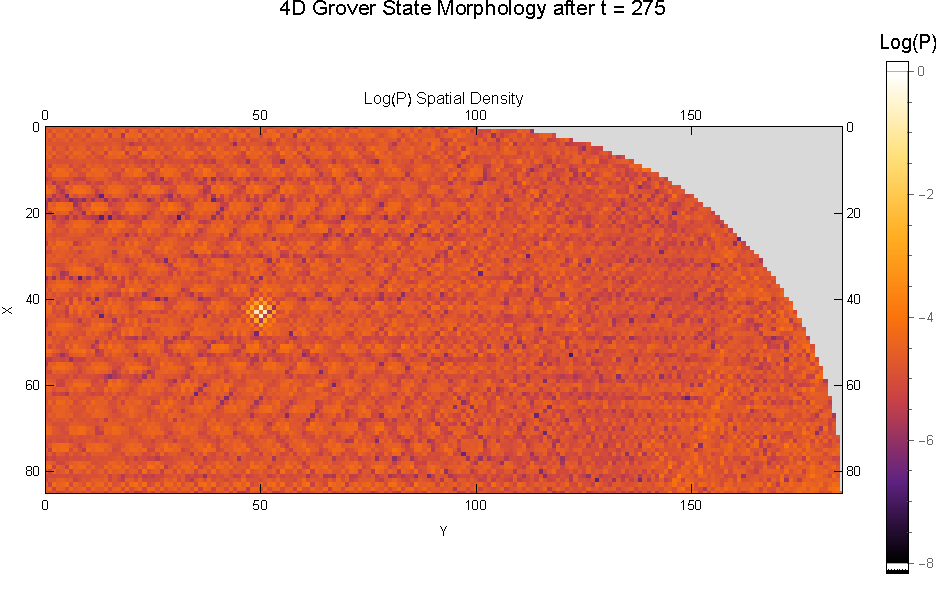
\includegraphics[width=0.8\textwidth]{BunimovichStateTimeEvol.pdf}
    \caption{Evolución de un estado localizado con estado inicial de moneda $(1,1,1,1)$ en el tiempo $t=275$ pasos. Dimensiones del estadio: $L=100$, $L_y=85$. Moneda de Grover: $\pi/4$.}
\end{figure}
\begin{figure}[H]
    \centering
    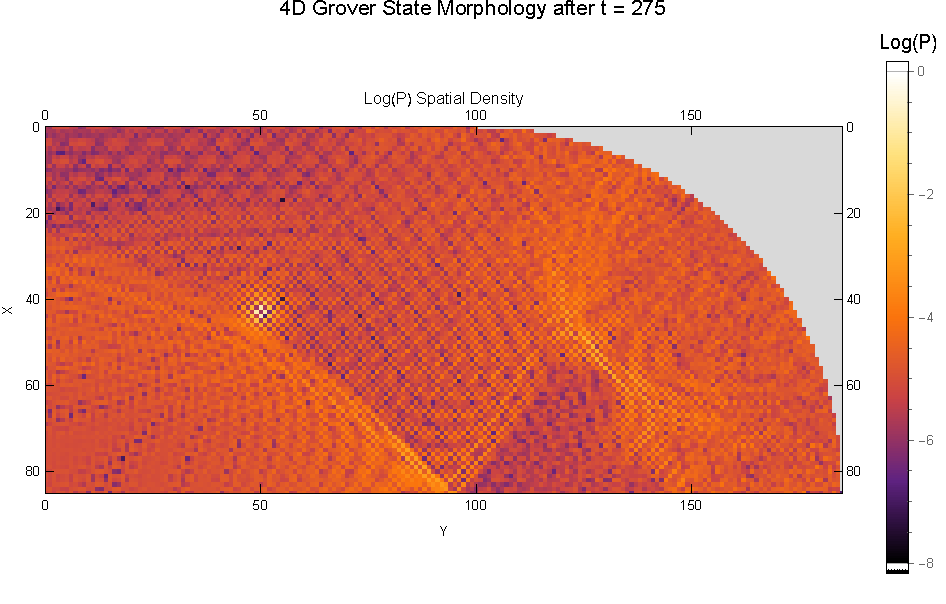
\includegraphics[width=0.8\textwidth]{BunimovichStateTimeEvolNonSymCoin.pdf}
    \caption{Evolución de un estado localizado con estado inicial de moneda $(1,-1,1,-1)$ en el tiempo $t=275$ pasos. Dimensiones del estadio: $L=100$, $L_y=85$. Moneda de Grover: $\pi/4$.}
\end{figure}

Hay un detalle que escapa a primera vista en el examen de estas figuras, y es lo mucho que cambia la distribución cuando el estado inicial de la moneda es $(1,1,1,1)$ en comparación a cuando no lo es.

Considere ahora las siguientes figuras en referencia a la evolución de un estado gaussiano:

\begin{figure}[H]
    \centering
     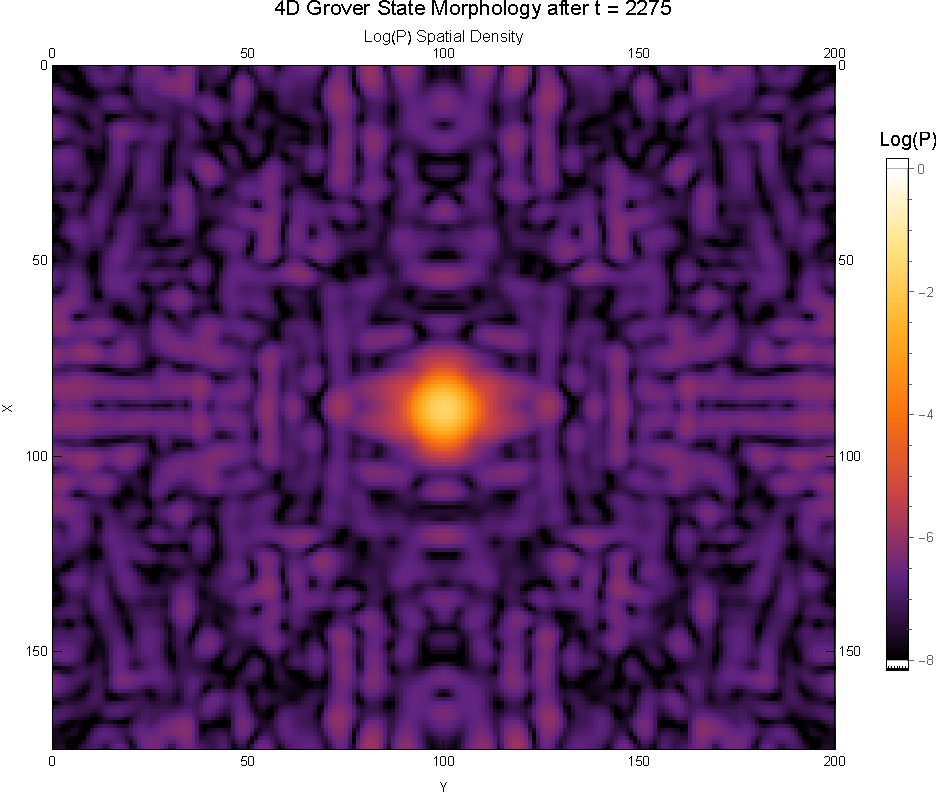
\includegraphics[width=0.7\textwidth]{RectangleGaussianStateTimeEvol.pdf}
    \caption{Evolución de un estado gaussiano con estado inicial de moneda $(1,1,1,1)$ en el tiempo $t=275$ pasos.}
\end{figure}
\begin{figure}[H]
    \centering
     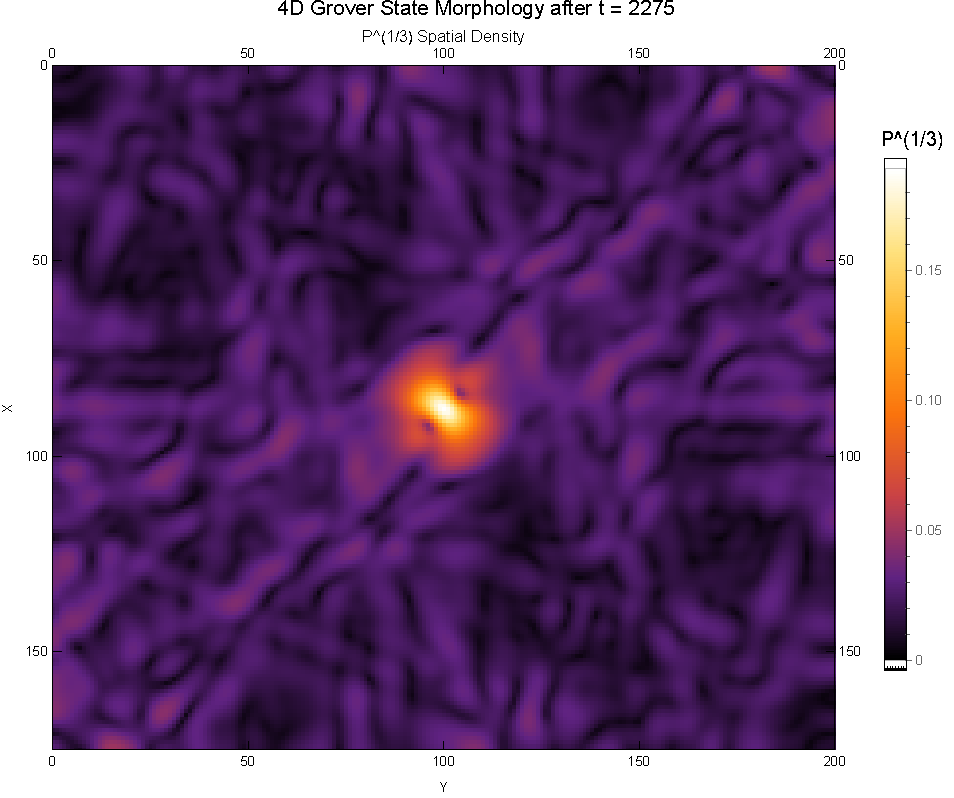
\includegraphics[width=0.7\textwidth]{RectangleGaussianStateTimeEvolNonSymCoin.pdf}
    \caption{Evolución de un estado gaussiano con estado inicial de moneda $(1,-1,1,-1)$ en el tiempo $t=275$ pasos.}
\end{figure}
\begin{figure}[H]
    \centering
     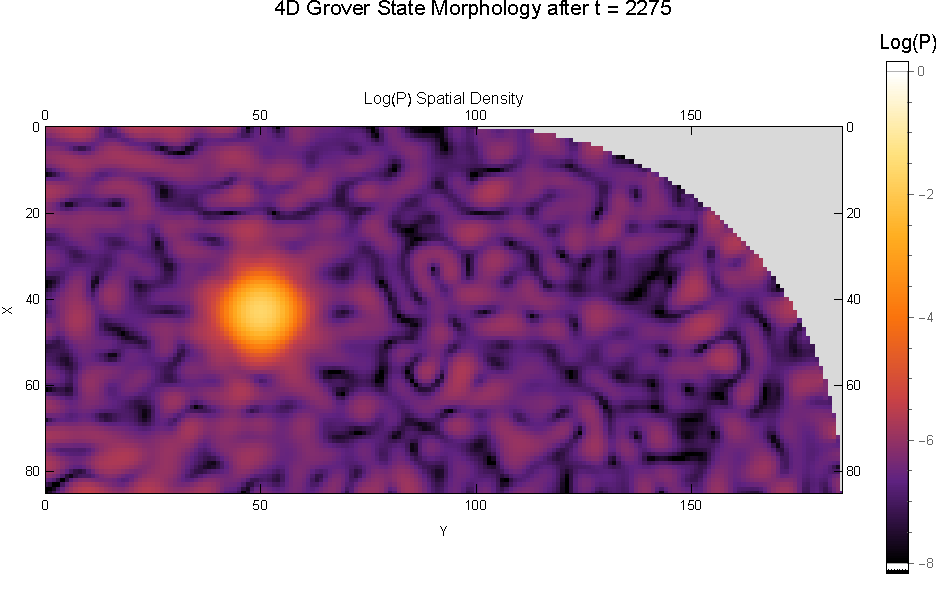
\includegraphics[width=0.7\textwidth]{BunimovichGaussianStateTimeEvol.pdf}
    \caption{Evolución de un estado gaussiano con estado inicial de moneda $(1,1,1,1)$ en el tiempo $t=2275$ pasos.}
\end{figure}
\begin{figure}[H]
    \centering
     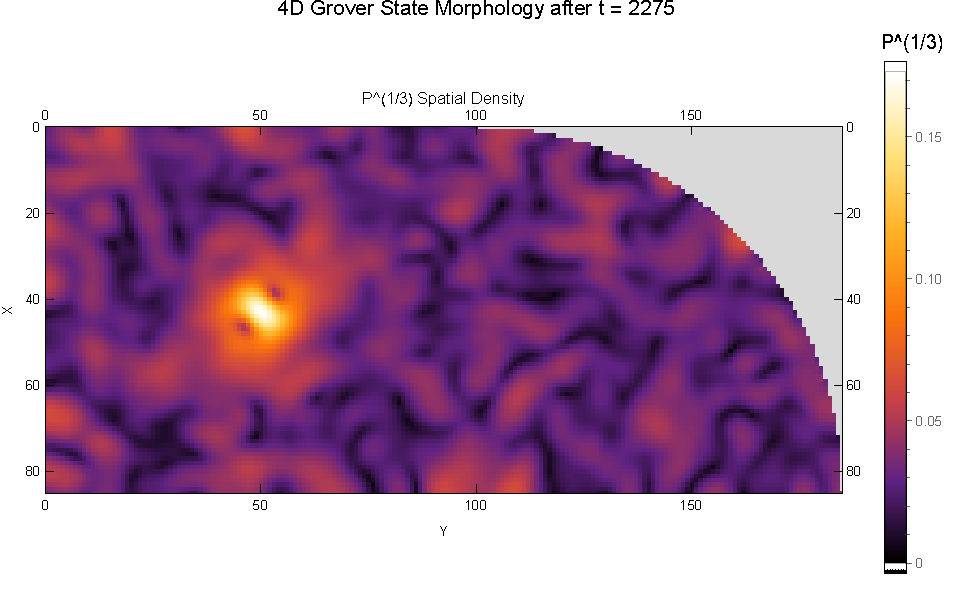
\includegraphics[width=0.7\textwidth]{BunimovichGaussianStateTimeEvolNonSymCoin.pdf}
    \caption{Evolución de un estado gaussiano con estado inicial de moneda $(1,-1,1,-1)$ en el tiempo $t=2275$ pasos.}
\end{figure}

Las figuras previas, tanto las de estados localizados como gaussianos, ponen en evidencia dos aspectos:

\begin{enumerate}
    \item El estado inicial de la moneda afecta significativamente la caminata. En particular, hay una diferencia sustancial entre usar un estado inicial de moneda (1,1,1,1) y utilizar uno que no lo sea.
    \item Se observa que la evolución del caminante para un estadio rectangular presenta patrones más 'ordenados' que los observados en el estadio de Bunimovich.
\end{enumerate}

\section{IPR espacial}

Vale la pena indagar más en cuantificar qué tan "localizado" se encuentra el caminante a medida que evoluciona. Por tanto, se considera la cantidad definida según:

\begin{equation}
    \text{IPR}_{\text{espacial}} = \frac{\sum_{i=1}^{N}P_{i}^{2}}{\left(\sum_{i=1}^{N}P_{i}\right)^{2}} = \frac{\sum_{i=1}^{N}\left(\sum_{c=1}^{4}|\Psi_{i,c}|^{2}\right)^{2}}{\left(\sum_{i=1}^{N}\sum_{c=1}^{4}|\Psi_{i,c}|^{2}\right)^{2}}
\end{equation}

Para cada posición espacial hay cuatro componentes en la moneda, por ello se realiza la suma sobre $c$. Se esperaría que, para distribuciones de probabilidad que muestren alguna concentración o localización, se magnifique su contribución; y que, para geometrías integrables, el valor del IPR sea mayor al visto con geometrías caóticas. 

A continuación, se muestran algunas curvas obtenidas para el IPR con la geometría rectangular empleando únicamente estados localizados en la posición.

\begin{figure}[H]
    \centering
     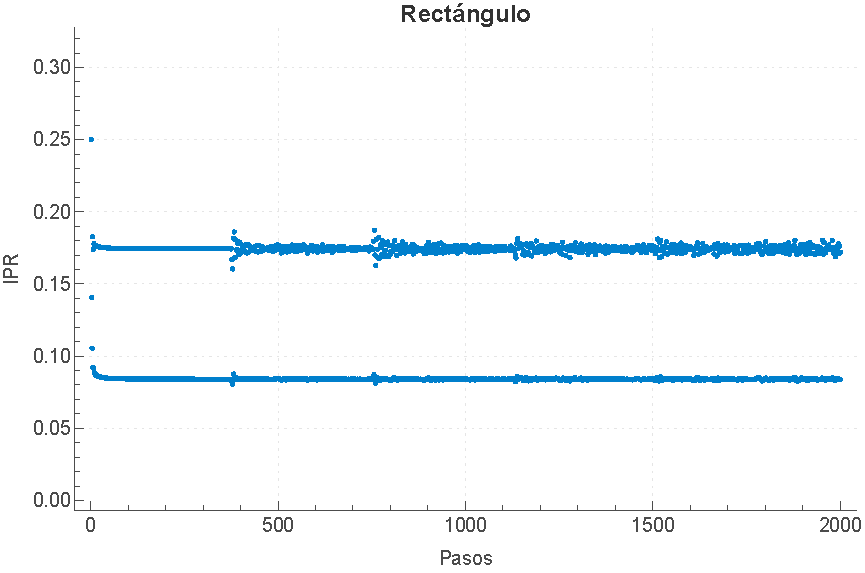
\includegraphics[width=0.7\textwidth]{RectangleLocalizedIPRNonSym.pdf}
    \caption{IPR hasta $t= 2000$, usando un estado localizado con estado inicial de moneda $(1,-1,1,-1)$. Las dimensiones del estadio son: $L_x=200$, $L_y= 175$. Ángulo de Grover: $\pi/4$.}
\end{figure}
\begin{figure}[H]
    \centering
     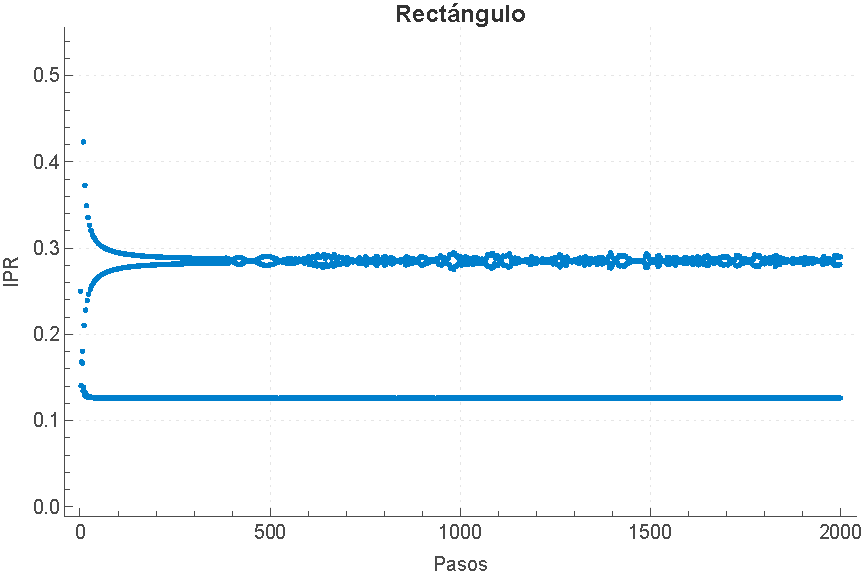
\includegraphics[width=0.7\textwidth]{RectangleLocalizedIPR.pdf}
    \caption{IPR hasta $t= 2000$, usando un estado localizado con estado inicial de moneda $(1,1,1,1)$. Las dimensiones del estadio son: $L_x=200$, $L_y= 175$. Ángulo de Grover: $\pi/4$.}
\end{figure}

Es de notar que un estado inicial de moneda que no es (1,1,1,1) se produce diferencias respecto a un estado que lo sea; nótese la presencia de "picos" cuando el estado de la moneda es $(1,-1,1,-1)$.

La presencia de las dos ramas observadas sugiere una relación entre los tiempos de evolución pares e impares. Siguiendo esta intuición, se separó el IPR para dichos tiempos, obteniendo el resultado esperado: 

\begin{figure}[H]
    \centering
     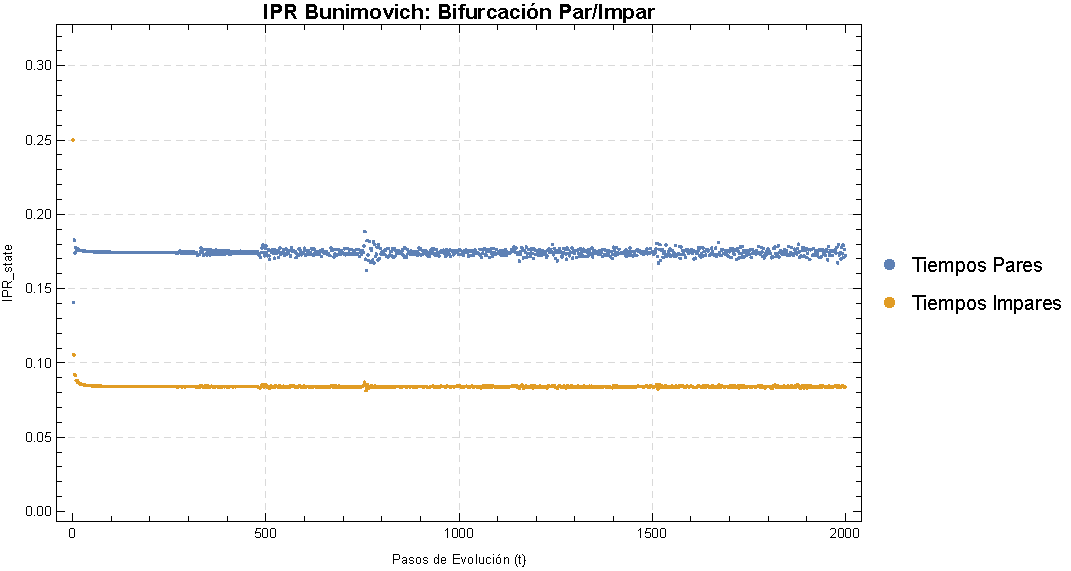
\includegraphics[width=0.7\textwidth]{RectangleLocalizedParityIPRNonSym.pdf}
    \caption{IPR hasta $t= 2000$, usando un estado localizado con estado inicial de moneda $(1,-1,1,-1)$. Las dimensiones del estadio rectangular son: $L_x=200$, $L_y= 175$. Ángulo de Grover: $\pi/4$. Datos separados en tiempos pares e impares.}
\end{figure}

Enfocándose en un estado inicial de moneda $(1,-1,1,-1)$, se examina por separado cada conjunto de tiempos:

\begin{figure}[h]
    \centering
     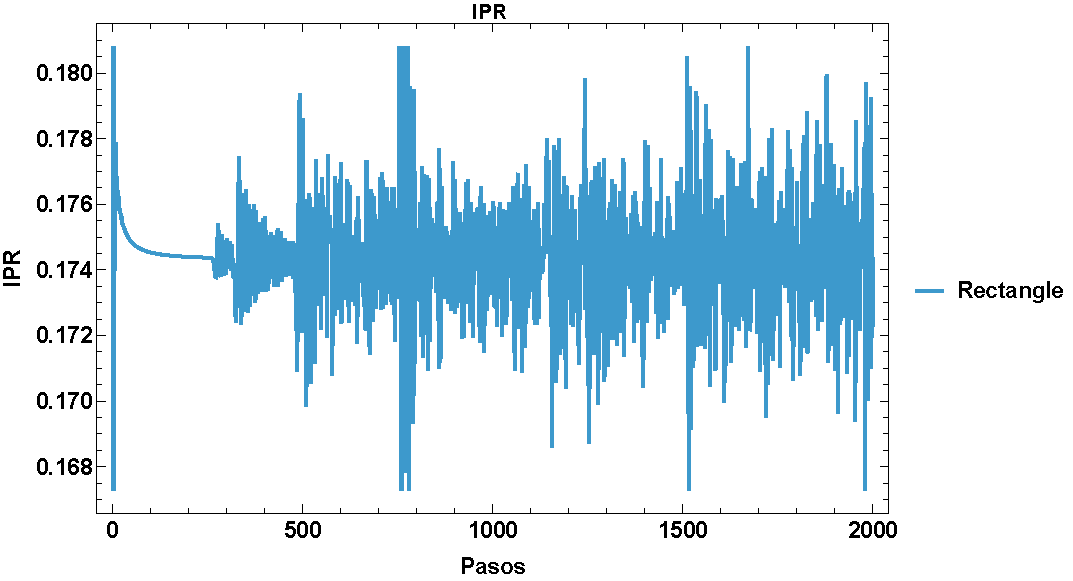
\includegraphics[width=0.7\textwidth]{RectangleLocalizedParityEvenIPRSym.pdf}
    \caption{Rama Par.}
\end{figure}
\begin{figure}[H]
    \centering
     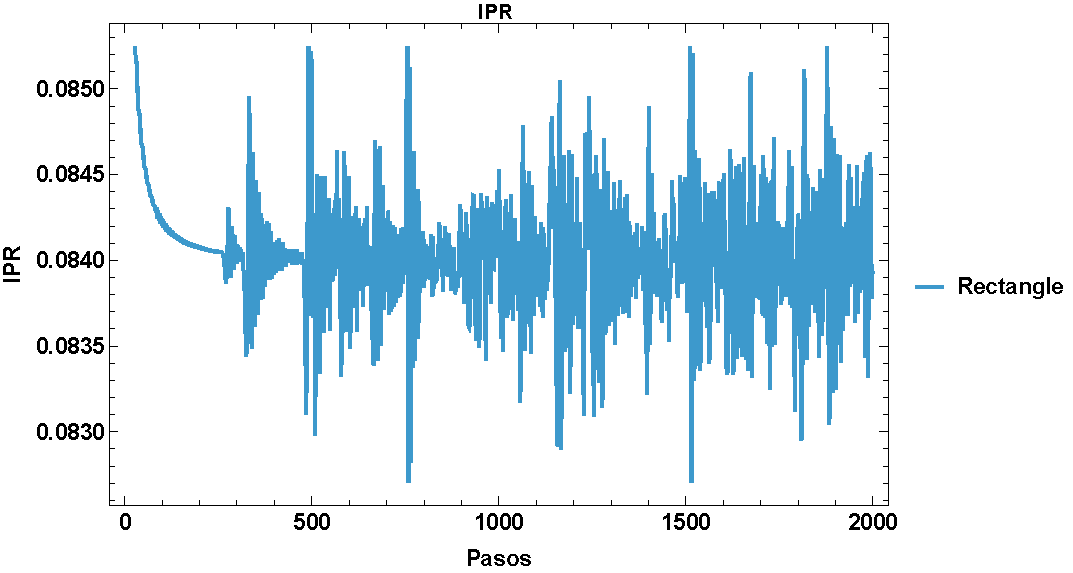
\includegraphics[width=0.7\textwidth]{RectangleLocalizedParityOddIPRSym.pdf}
    \caption{Rama Impar.}
\end{figure}

Cabe enfatizar que el uso de un estado inicial de moneda no simétrico permite observar, para cada rama del IPR, la existencia de picos a intervalos de tiempo regulares. ¿Son estos picos detectables en el estadio de Bunimovich, empleando el mismo estado inicial de la moneda y dimensiones comparables?

\begin{figure}[H]
    \centering
     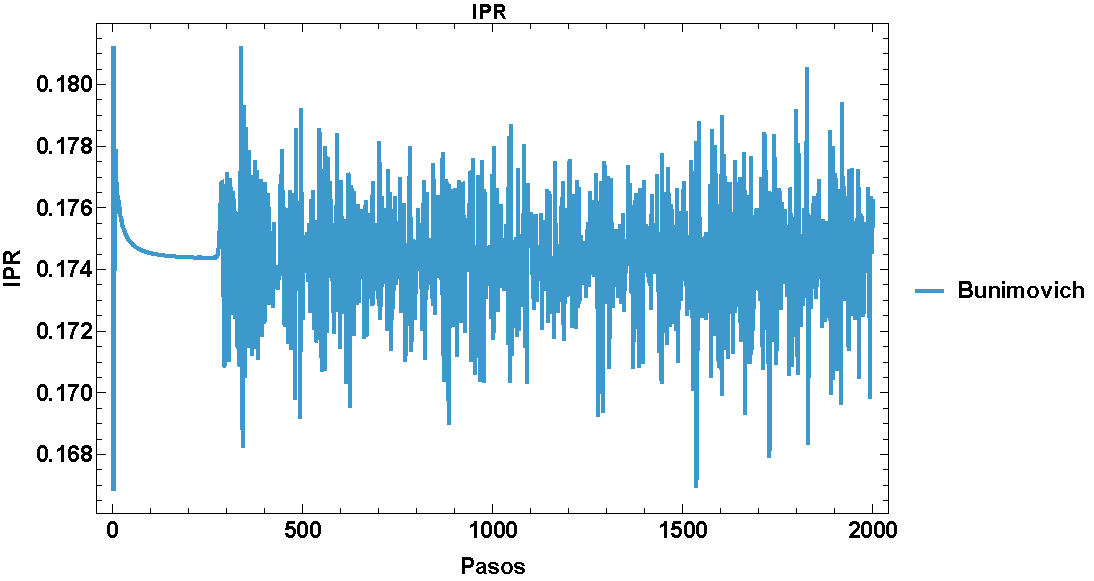
\includegraphics[width=0.7\textwidth]{BunimovichLocalizedParityEvenIPRNonSym.pdf}
    \caption{Rama Par de un estadio Bunimovich de dimensiones $L=90$ y $R= 65$. }
\end{figure}
\begin{figure}[H]
    \centering
     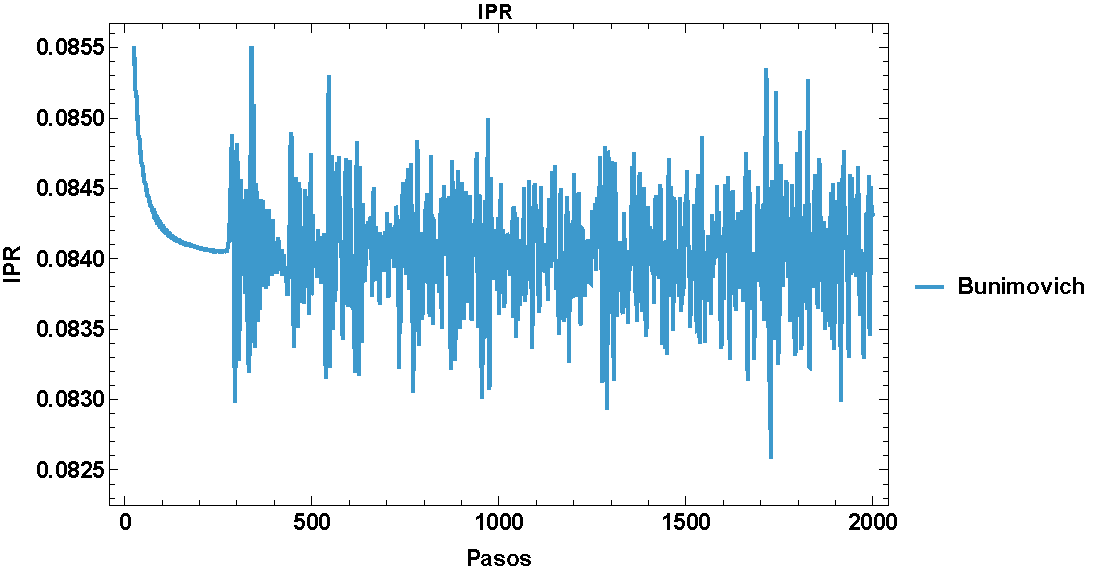
\includegraphics[width=0.7\textwidth]{BunimovichLocalizedParityOddIPRNonSym.pdf}
    \caption{Rama Impar de un estadio Bunimovich de dimensiones $L=90$ y $R= 65$.}
\end{figure}

Se observa que tanto en el rectángulo como en el estadio de Bunimovich existe la presencia de estos 'picos'; sin embargo, cualitativamente, los picos observados en el rectángulo tienen mayor amplitud. Usando dimensiones comparables (áreas aproximadas), se observa lo siguiente:

\begin{figure}[H]
    \centering
     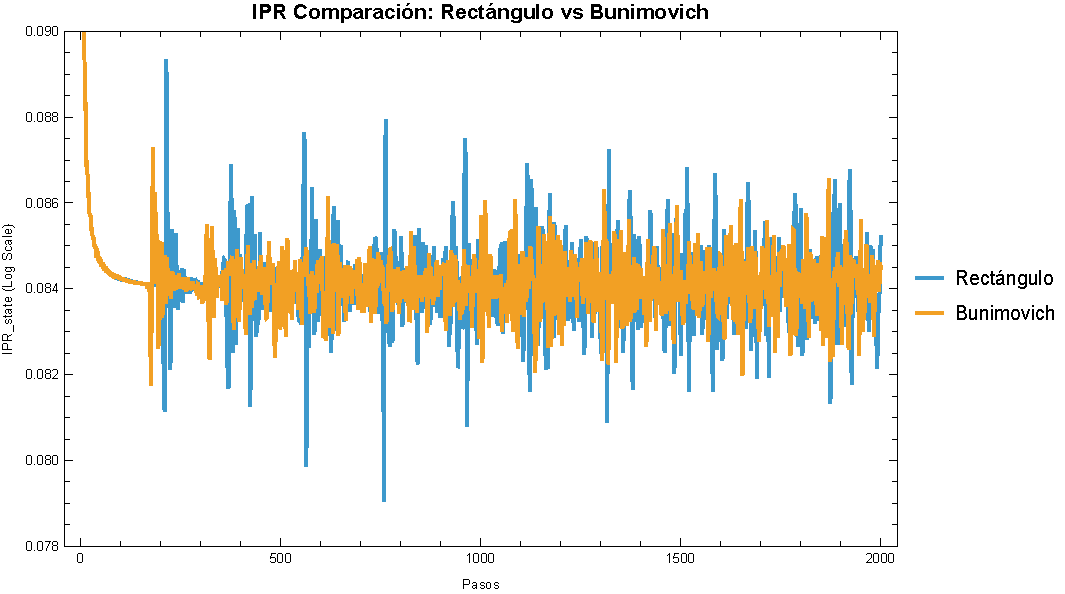
\includegraphics[width=0.7\textwidth]{ComparativeLocalizedParityEvenIPRNonSym.pdf}
    \caption{Rama Par. Las dimensiones del rectángulo son $L_x= 125$, $L_y= 75$. Las dimensiones de Bunimovich son $L=90$, $R= 65$.}
\end{figure}
\begin{figure}[H]
    \centering
     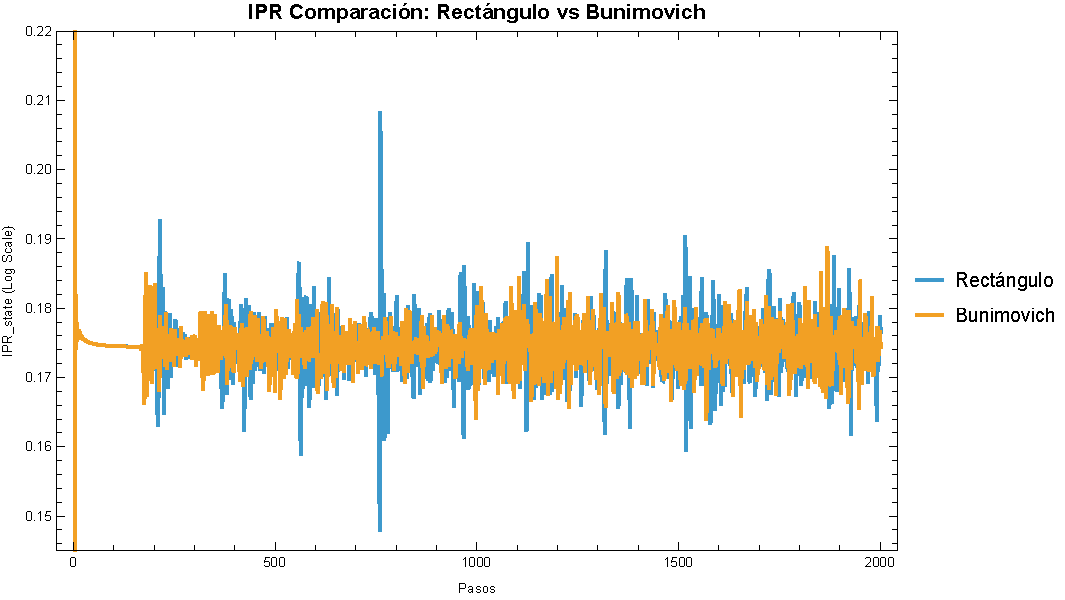
\includegraphics[width=0.7\textwidth]{ComparativeLocalizedParityOddIPRNonSym.pdf}
    \caption{Rama Impar. Las dimensiones del rectángulo son $L_x= 125$, $L_y= 75$. Las dimensiones de Bunimovich son $L=90$, $R= 65$.}
\end{figure}

Vale la pena indagar un poco más sobre estos picos en el caso del rectángulo:

\begin{figure}[H]
    \centering
     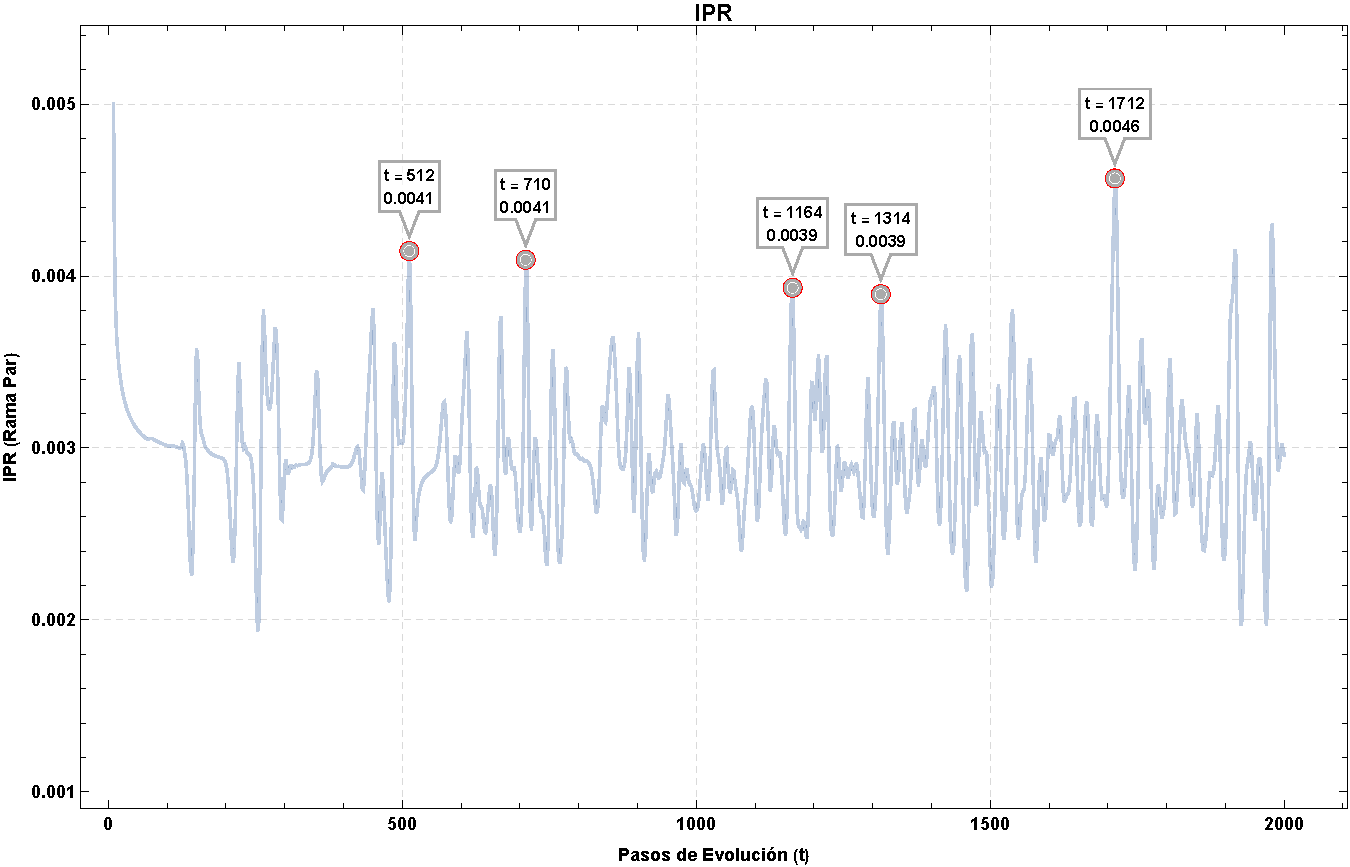
\includegraphics[width=0.7\textwidth]{PeaksPointsRectangleGaussianParityEvenIPRNonSym.pdf}
    \caption{Picos detectados para el rectángulo con dimensiones $L_x=150$, $L_y= 100$, para un estado localizado con estado inicial de moneda $(1,-1,1,-1)$.}
\end{figure}

Para este estadio en particular y estado inicial del caminante, se obtuvo que los picos suceden en los tiempos: $(4, 262, 524, 778, 974, 1214, 1472, 1712)$. Con esto se puede determinar que cada pico ocurre cada 244 pasos con una incertidumbre de 23 pasos. 

Trabajando con la rama impar, se obtiene que los picos suceden en los tiempos: $(1, 261, 487, 777, 963, 1209, 1471, 1737, 1919)$, donde cada pico ocurre cada 240 pasos con una incertidumbre de 39 pasos. 

Si se emplea un tamaño de estadio más grande, ¿se podrá ver con mayor precisión este aparente período en la aparición de los picos? Para ello se consideraron dimensiones de $L_x=350$ y $L_y=200$, calculando hasta un tiempo $t=6000$ con un estado inicial localizado. No se obtuvo una reducción en la incertidumbre; se sigue observando el mismo comportamiento pero con tiempos distintos, lo que sugiere que la periodicidad de estos picos depende directamente del tamaño de la geometría.

¿ Realmente hay una periodicidad en los picos ? 

Examinaré cada rama (par e impar) por separado, y veré si, mediante una operación de $mod \, n$ se puede obtener más información acerca de los picos.
Emplearé primero un estadio rectangular de dimensiones $L_x=200 \, , L_y=175$, un estado localizado, que empice en el centro del estadio y estado inicial de moneda $(1,-1,1,-1)$.

Para la rama par:
    \begin{figure}[H]
\centering
    % --- Primera Subfigura ---
\begin{subfigure}[b]{0.8\textwidth}
\centering
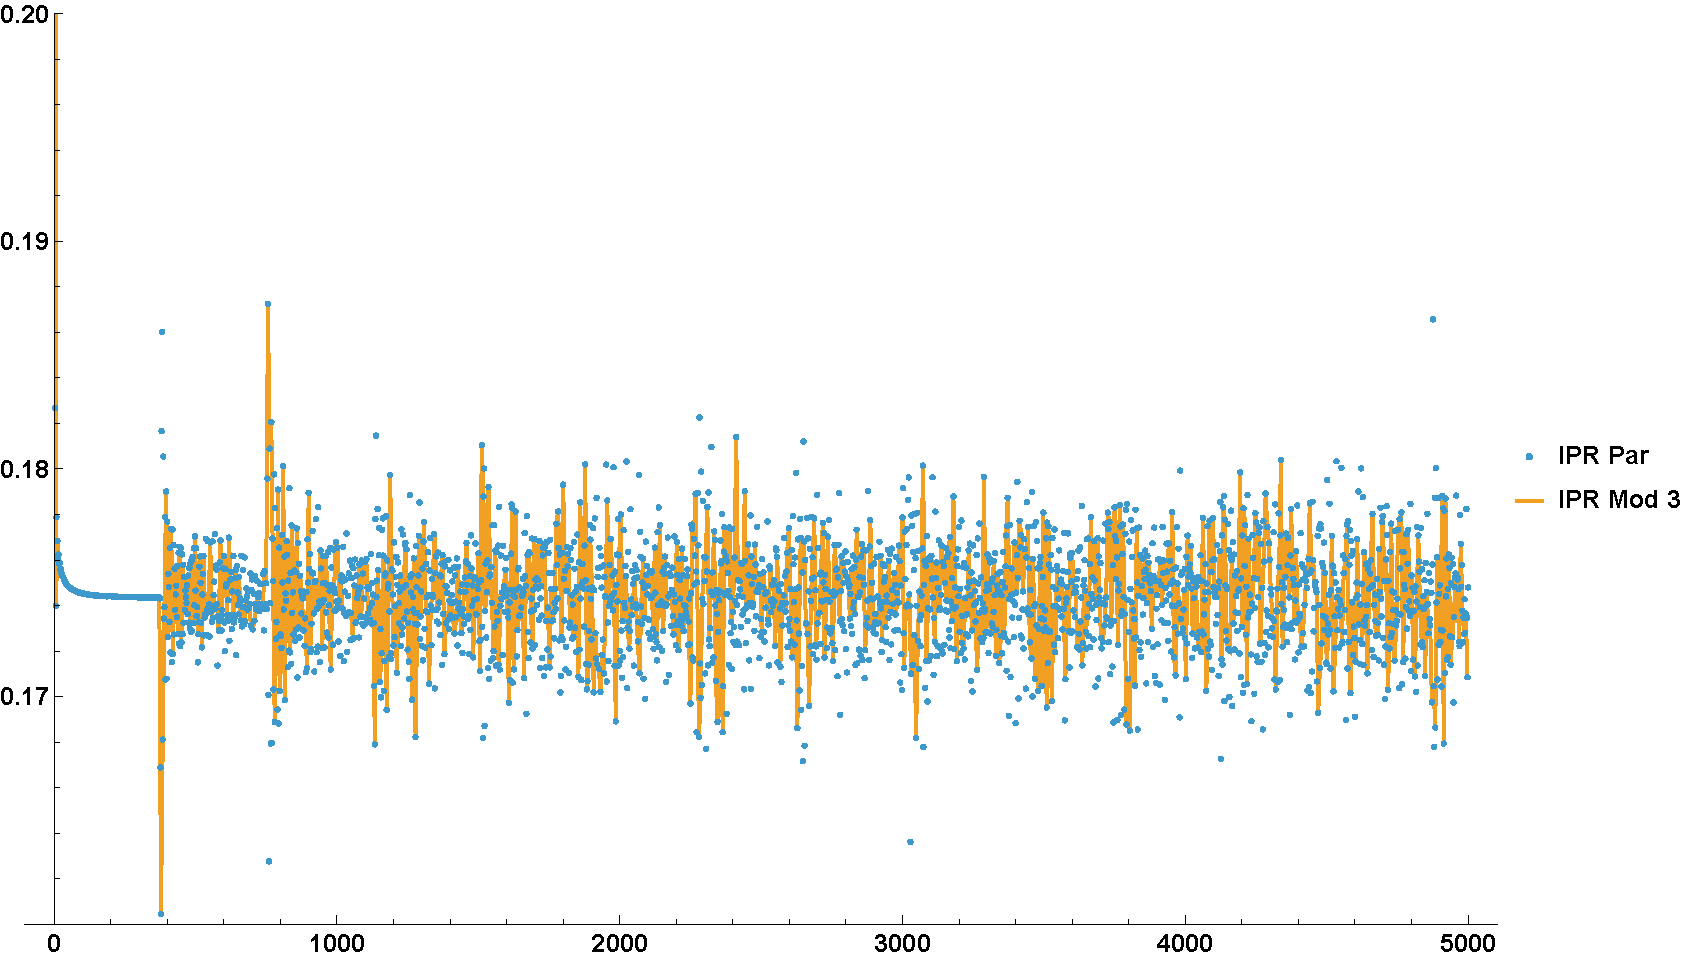
\includegraphics[width=0.8\textwidth]{IPRRectEvenMod3.pdf}
\caption{Rama par para tiempos $mod \,  3$}
\label{fig:mod3}
\end{subfigure}
\hfill % Agrega un espacio flexible entre las dos imágenes
    % --- Segunda Subfigura ---
\begin{subfigure}[b]{0.8\textwidth}
\centering
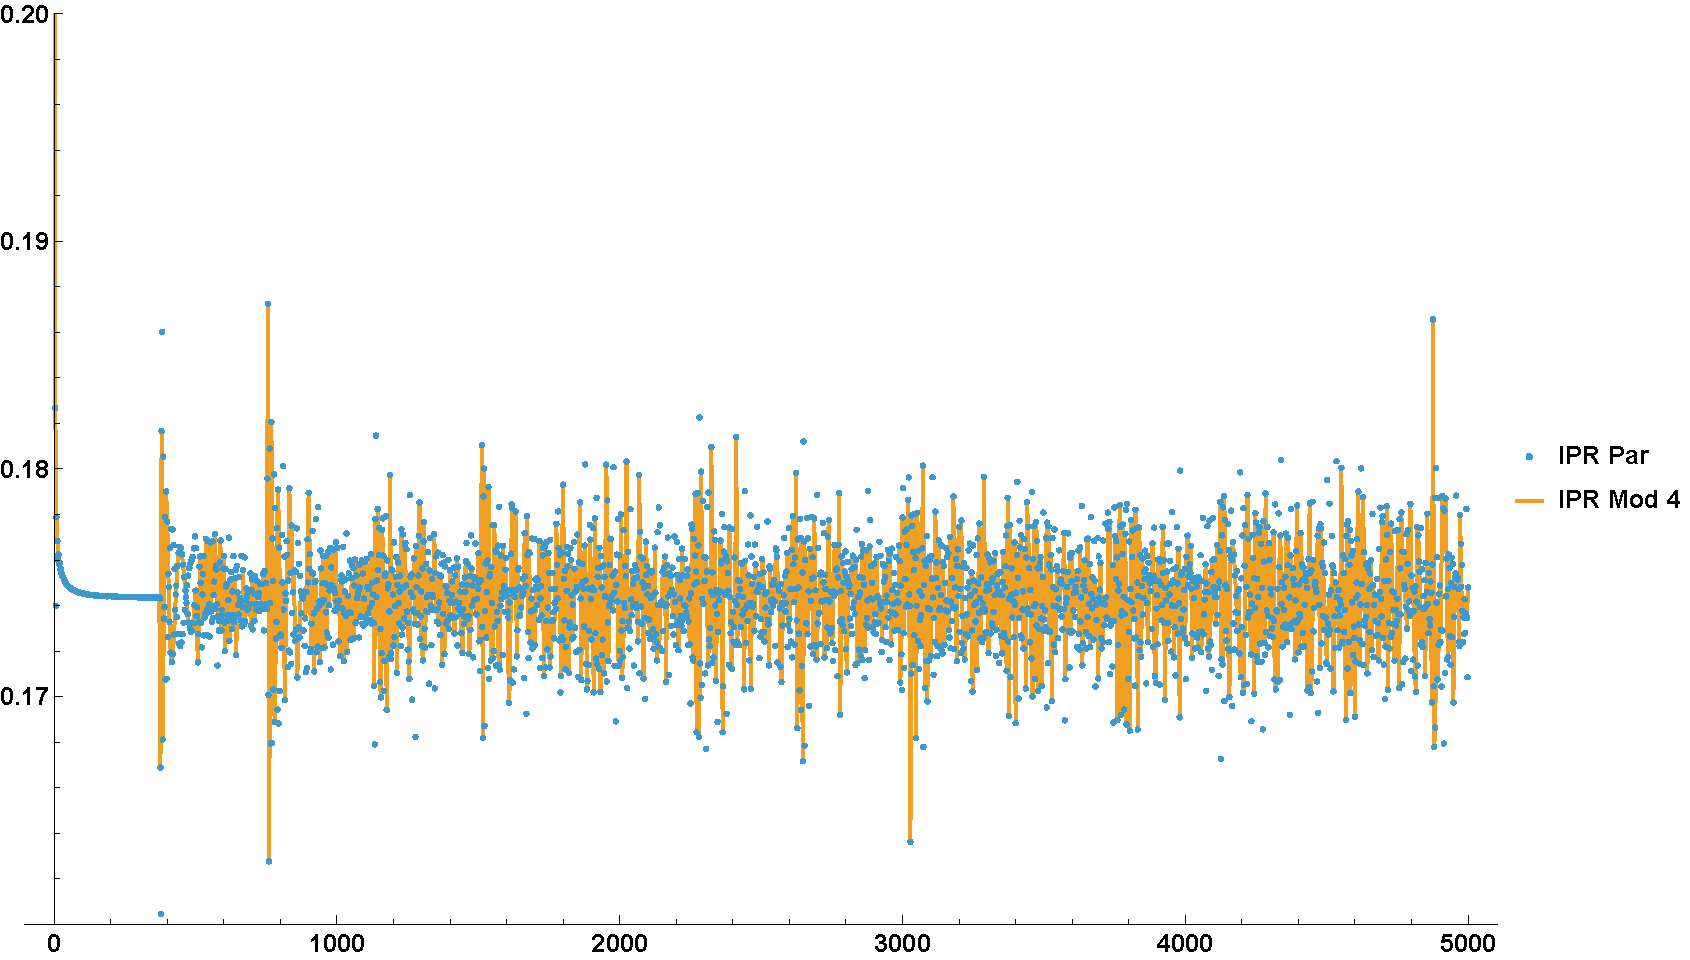
\includegraphics[width=0.8\textwidth]{IPRRectEvenMod4.pdf}
\caption{Rama par para tiempos $mod \,  4$}
\label{fig:Mod4}
\end{subfigure}
\begin{subfigure}[b]{0.8\textwidth}
\centering
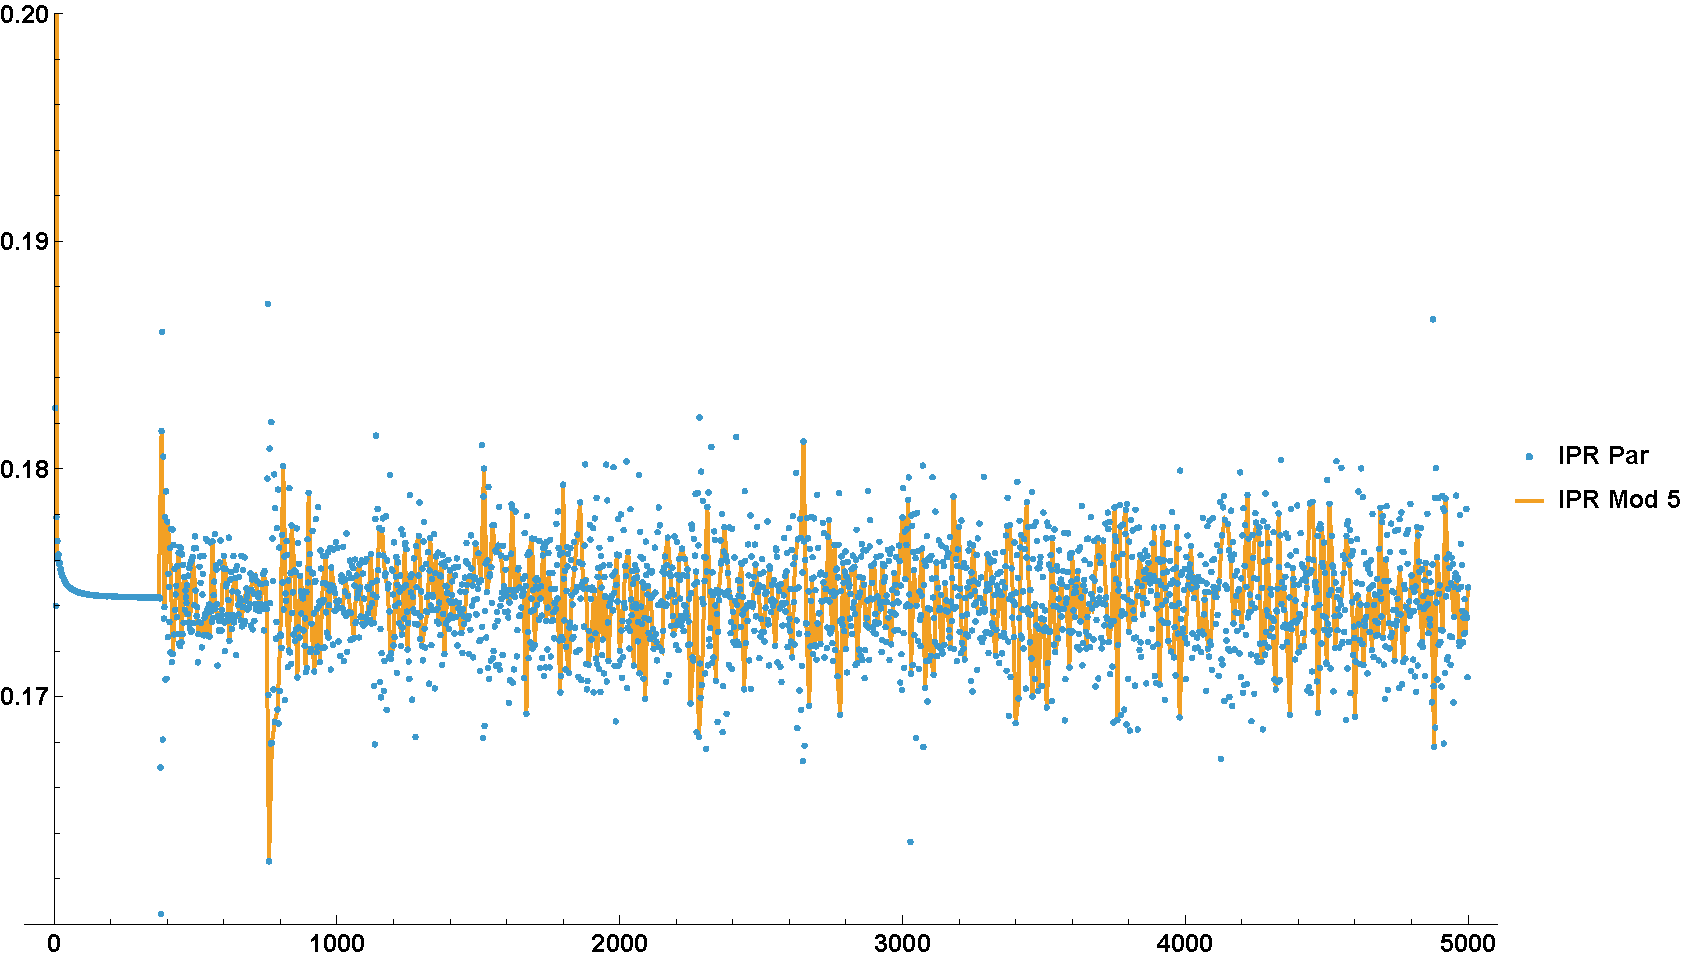
\includegraphics[width=0.8\textwidth]{IPRRectEvenMod5.pdf}
\caption{Rama par para tiempos $mod \,  5$}
\label{fig:Mod5}
\end{subfigure}
\end{figure}
   

Para tiempos enteros, $t=(p_1)^{k_1}\cdot...\cdot (p_m)^{k_m}$, siendo $p_i$ números primos y $k_i\in \mathbb{N}$

 \begin{figure}[H]
\centering
    % --- Primera Subfigura ---
\begin{subfigure}[b]{0.8\textwidth}
\centering
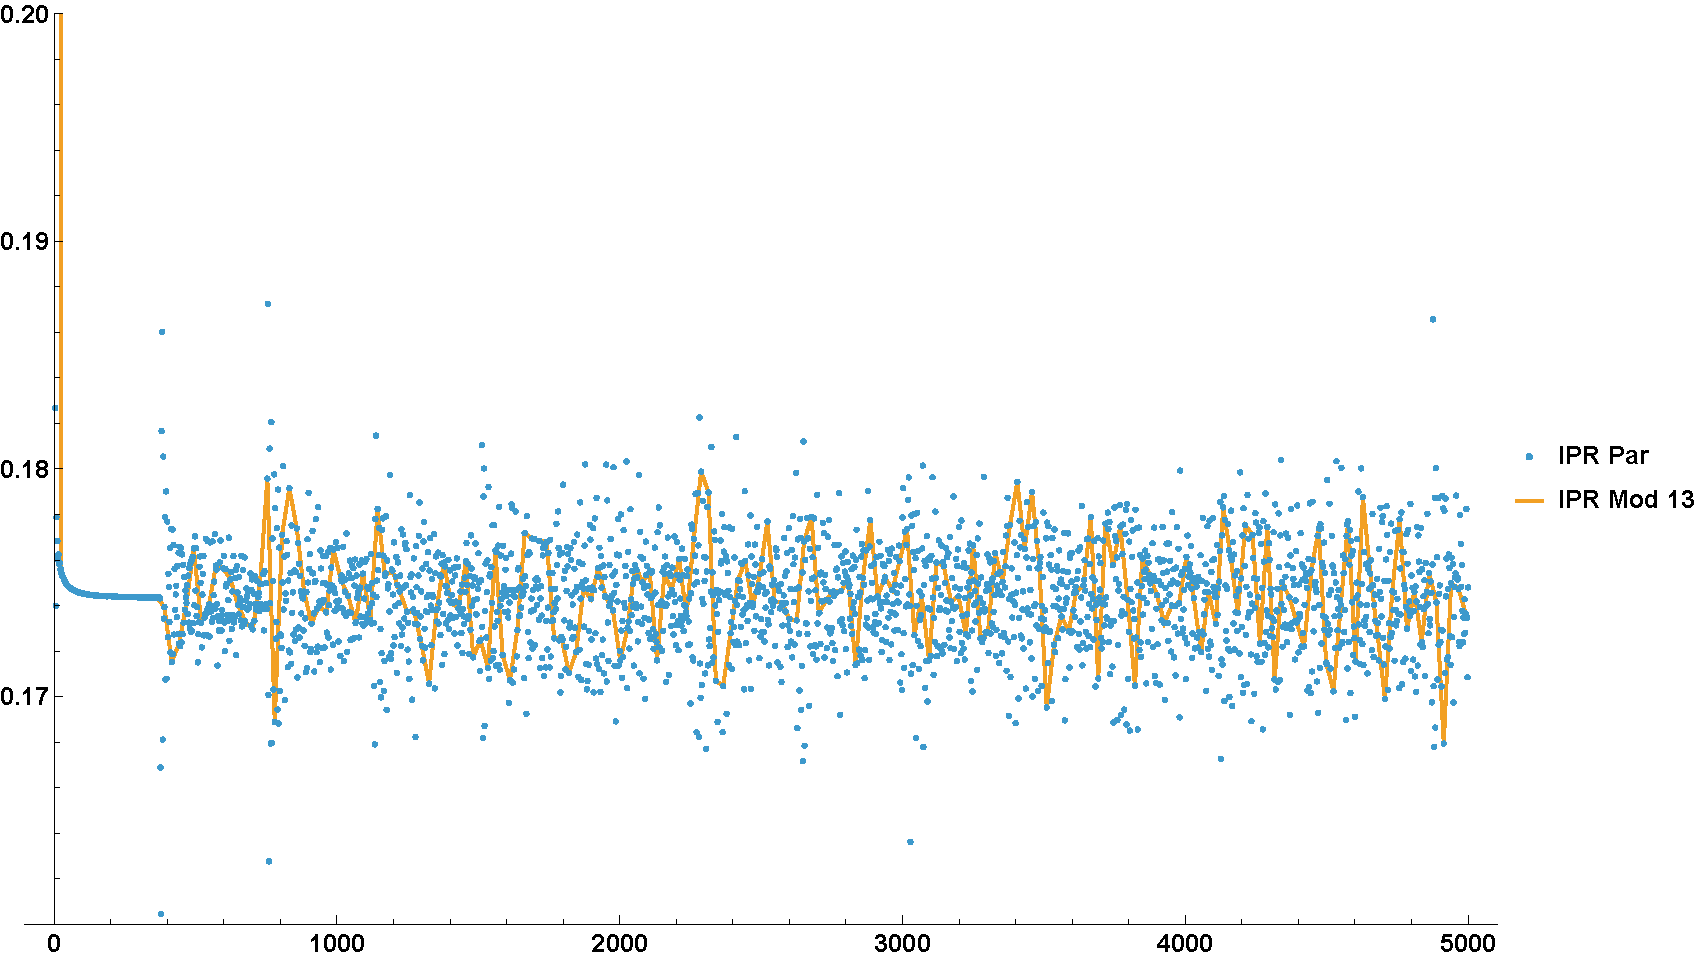
\includegraphics[width=0.8\textwidth]{IPRRectEvenMod13.pdf}
\caption{Rama par para tiempos $mod \,  13$}
\label{fig:mod13}
\end{subfigure}
\hfill % Agrega un espacio flexible entre las dos imágenes
    % --- Segunda Subfigura ---
\begin{subfigure}[b]{0.8\textwidth}
\centering
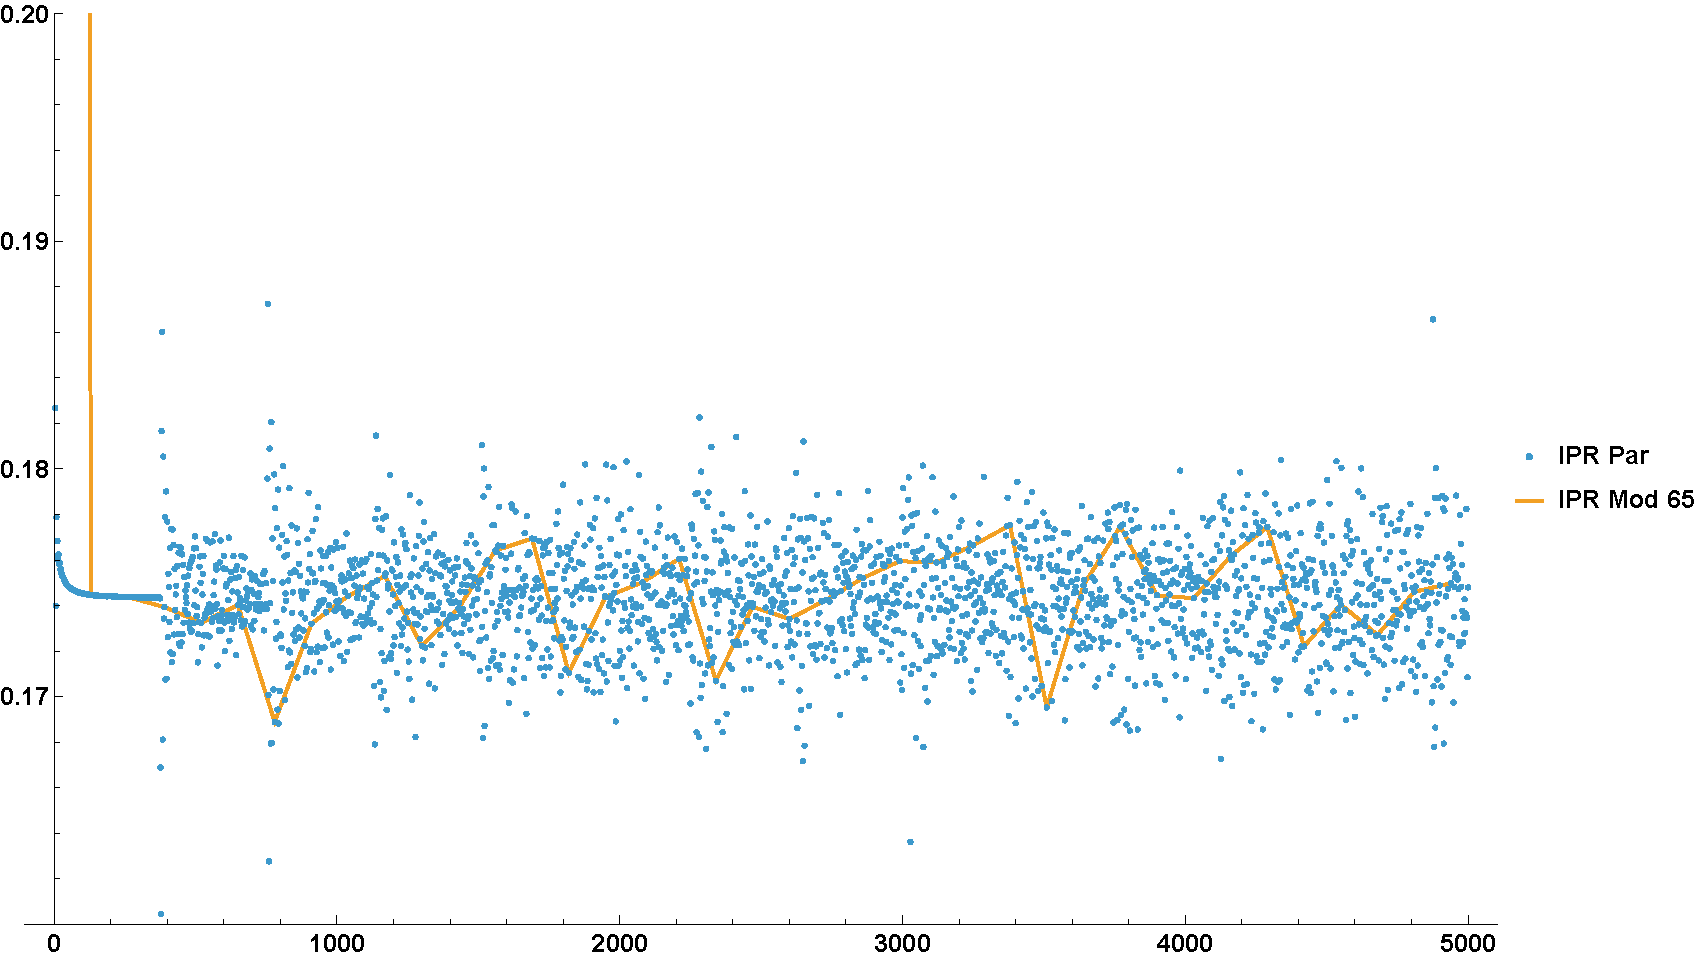
\includegraphics[width=0.8\textwidth]{IPRRectEvenMod13tim5.pdf}
\caption{Rama par para tiempos $mod \,  13\cdot5$}
\label{fig:Mod13tim5}
\end{subfigure}
\begin{subfigure}[b]{0.8\textwidth}
\centering
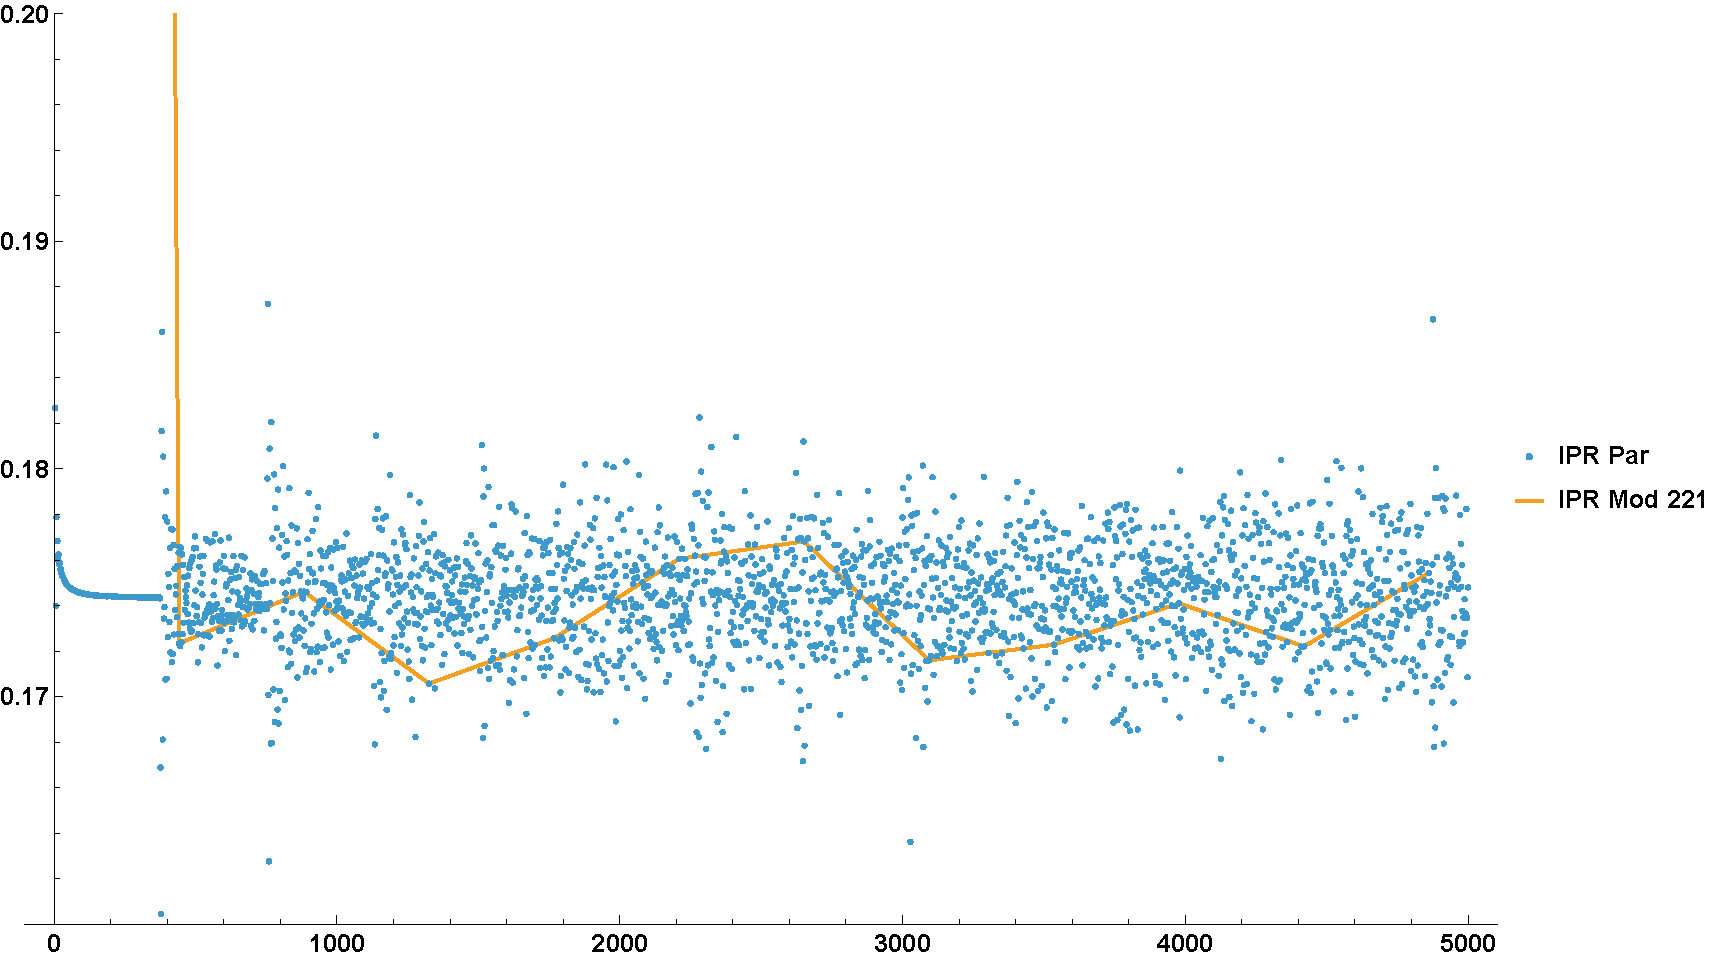
\includegraphics[width=0.8\textwidth]{IPRRectEvenMod13tim17.pdf}
\caption{Rama par para tiempos $mod \,  5\cdot 17$}
\label{fig:Mod13tim17}
\end{subfigure}
\end{figure}

Un detalle que me parece importante señalar es que, para estos tiempos, se ve que la IPR parece oscilar en hasta una amplitud máxima.
Vale la pena observar al caminante en saltos de $t=(p_1)^{k_1}\cdot...\cdot (p_m)^{k_m}$.

\section{Sobre la propagación del caminante según su moneda}

Según las figuras mostradas previamente, no resulta concluyente afirmar si la propagación del caminante es balística, por lo que se calcula la desviación estándar definida como: 

\begin{equation}
    \sigma = \sqrt{(\langle x^{2}\rangle - \langle x\rangle^{2}) + (\langle y^{2}\rangle - \langle y\rangle^{2})}
\end{equation}

La propagación es balística si $\sigma \propto t$. 

Considerando un estadio rectangular con dimensiones $L_x=250$ y $L_y=200$, empleando un ángulo de grover de $\frac{\pi}{4}$, se muestra como varía $\sigma$ según la evolución de diferentes estados iniciales.

\begin{figure}[H]
\centering
    % --- Primera Subfigura ---
\begin{subfigure}[b]{0.45\textwidth}
\centering
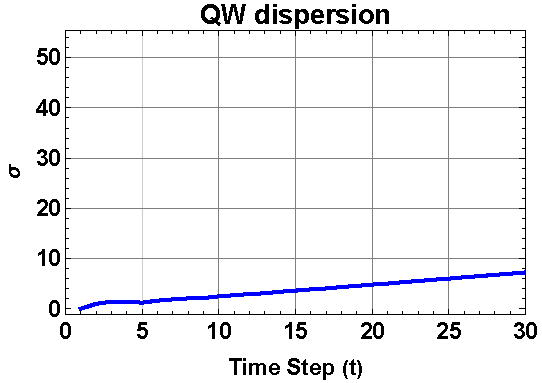
\includegraphics[width=\textwidth]{std_Pi_4_SymCenterT30.pdf}
\caption{Hasta $t= 30$.}
\label{fig:izq1}
\end{subfigure}
\hfill % Agrega un espacio flexible entre las dos imágenes
    % --- Segunda Subfigura ---
\begin{subfigure}[b]{0.45\textwidth}
\centering
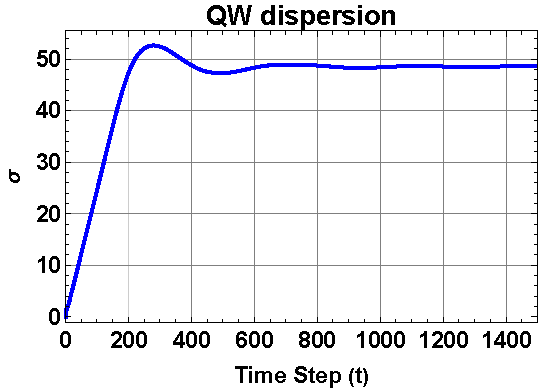
\includegraphics[width=\textwidth]{std_Pi_4_SymCenterT150.pdf}
\caption{Hasta $t= 1500$.}
\label{fig:der1}
\end{subfigure}
    
\caption{Estado localizado en la posición $(125,100)$, con estado inicial de moneda $(1,1,1,1)$}
\label{fig:ambas1}
\end{figure}


\begin{figure}[H]
\centering
    % --- Primera Subfigura ---
\begin{subfigure}[b]{0.45\textwidth}
\centering
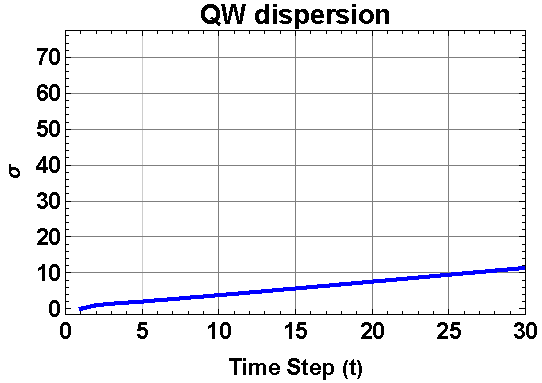
\includegraphics[width=\textwidth]{std_Pi_4_NonSymCenterT30.pdf}
\caption{Hasta $t= 30$.}
\label{fig:izq2}
\end{subfigure}
\hfill % Agrega un espacio flexible entre las dos imágenes
    % --- Segunda Subfigura ---
\begin{subfigure}[b]{0.45\textwidth}
\centering
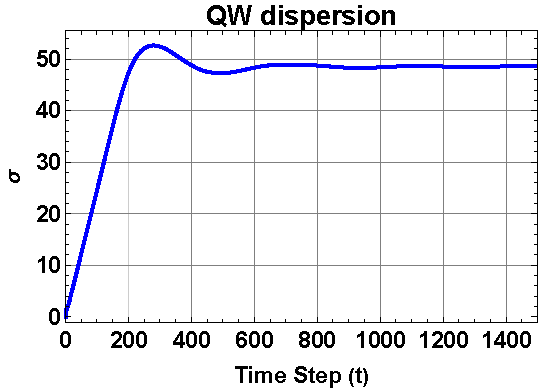
\includegraphics[width=\textwidth]{std_Pi_4_SymCenterT150.pdf}
\caption{Hasta $t= 1500$.}
\label{fig:der2}
\end{subfigure}
    
\caption{Estado localizado en la posición $(125,100)$, con estado inicial de moneda $(1,-1,1,-1)$}
\label{fig:ambas2}
\end{figure}

\begin{figure}[H]
\centering
    % --- Primera Subfigura ---
\begin{subfigure}[b]{0.45\textwidth}
\centering
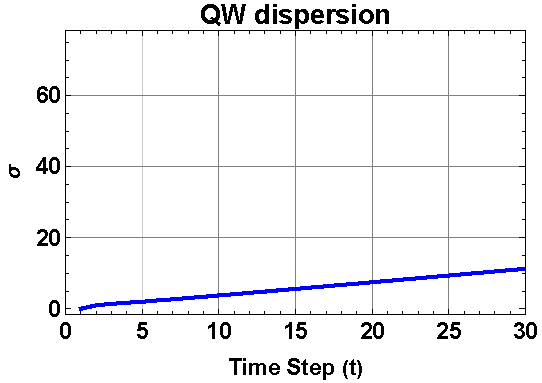
\includegraphics[width=\textwidth]{std_Pi_4_RandomStateT30.pdf}
\caption{Hasta $t= 30$.}
\label{fig:izq3}
\end{subfigure}
\hfill % Agrega un espacio flexible entre las dos imágenes
    % --- Segunda Subfigura ---
\begin{subfigure}[b]{0.45\textwidth}
\centering
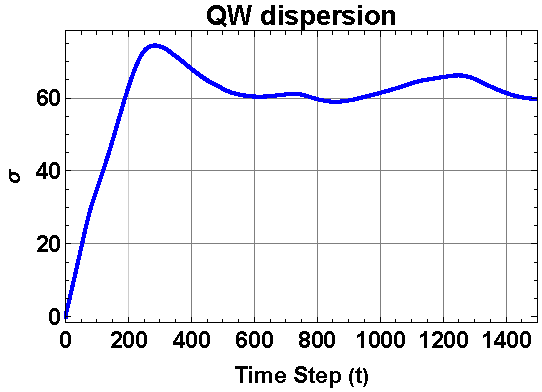
\includegraphics[width=\textwidth]{std_Pi_4_RandomStateT1500.pdf}
\caption{Hasta $t= 1500$.}
\label{fig:der3}
\end{subfigure}
    
\caption{Estado localizado en una posición aleatoria y con un estado de moneda aleatorio.}
\label{fig:ambas3}
\end{figure}

\begin{figure}[H]
\centering
    % --- Primera Subfigura ---
\begin{subfigure}[b]{0.45\textwidth}
\centering
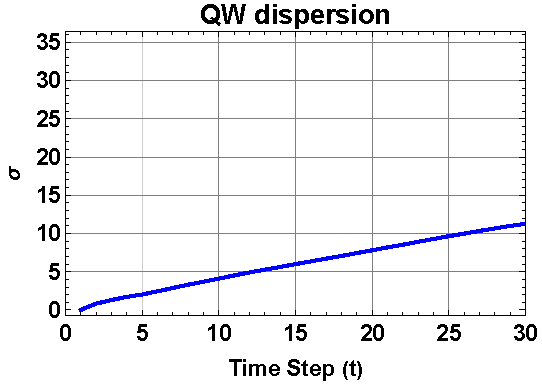
\includegraphics[width=\textwidth]{std_Pi_4_RandomStateT30Bun.pdf}
\caption{Hasta $t= 30$.}
\label{fig:izq4}
\end{subfigure}
\hfill % Agrega un espacio flexible entre las dos imágenes
    % --- Segunda Subfigura ---
\begin{subfigure}[b]{0.45\textwidth}
\centering
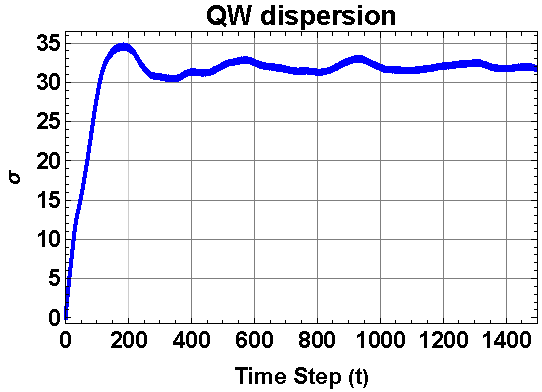
\includegraphics[width=\textwidth]{std_Pi_4_RandomStateT1500Bun.pdf}
\caption{Hasta $t= 1500$.}
\label{fig:der4}
\end{subfigure}
    
\caption{Estado localizado en una posición aleatoria y con un estado de moneda aleatorio emplenado un \textbf{estadio bunimovich con $L= 90\,, R= 65$}.}
\label{fig:ambas4}
\end{figure}

Es observado que, tanto para un estadio rectángular (clásicamente integrable) como un estadio del tipo bunimovich (clásicamente caótico),
la desviación estándar si satisface con $\sigma \propto t$, por lo menos para una ventana de tiempo dada.

Supongamos una venta de tiempo tal que $\sigma \propto t \, \rightarrow \sigma = \alpha t$, y podemos interpretar a $\alpha$ como una medida de "que tan rápido se mueve".
Me parece interesante comprobar si:
\begin{itemize}
    \item ¿ Qué estados iniciales son más 'rápidos' ?
    \item ¿ Cómo varía esta "rapidez" según el estadio a considerar ?
\end{itemize}
Primero, consideraré un estadio rectangular, de dimensiones $L_x= 200\, , L_y=150$.

\begin{figure}[H]
\centering
    % --- Primera Subfigura ---
\begin{subfigure}[b]{0.5\textwidth}
\centering
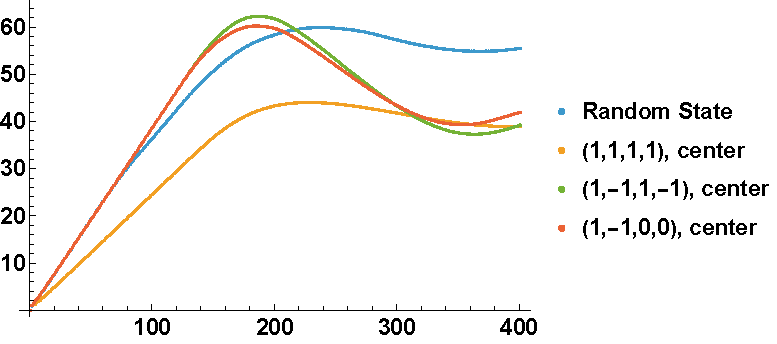
\includegraphics[width=\textwidth]{stdRectComp1.pdf}
\caption{}
\label{fig:izq5}
\end{subfigure}
\hfill % Agrega un espacio flexible entre las dos imágenes
    % --- Segunda Subfigura ---
\begin{subfigure}[b]{0.5\textwidth}
\centering
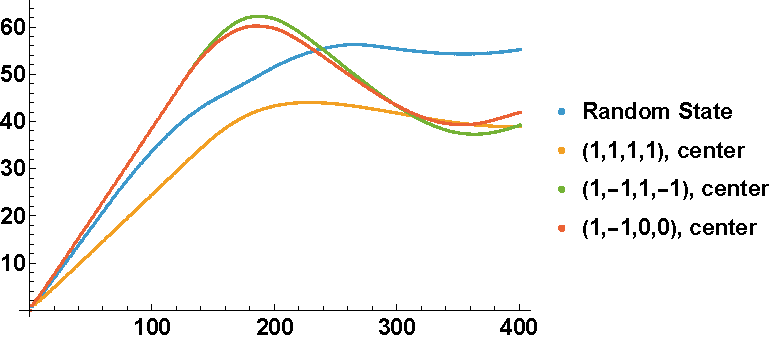
\includegraphics[width=\textwidth]{stdRectComp2.pdf}
\caption{}
\label{fig:der5}
\end{subfigure}

\begin{subfigure}[b]{0.5\textwidth}
\centering
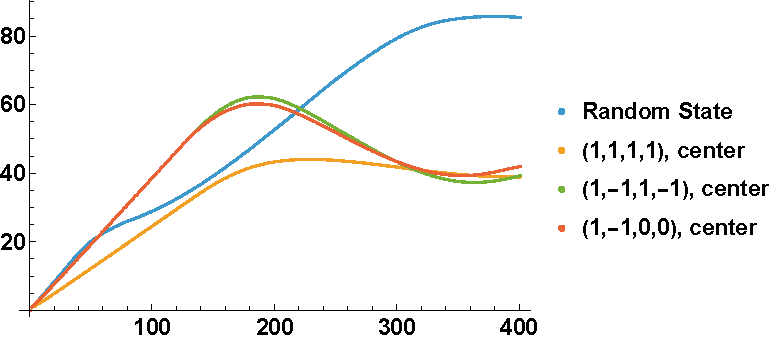
\includegraphics[width=\textwidth]{stdRectComp3.pdf}
\caption{}
\label{fig:izq6}
\end{subfigure}
\hfill % Agrega un espacio flexible entre las dos imágenes
    % --- Segunda Subfigura ---
\begin{subfigure}[b]{0.5\textwidth}
\centering
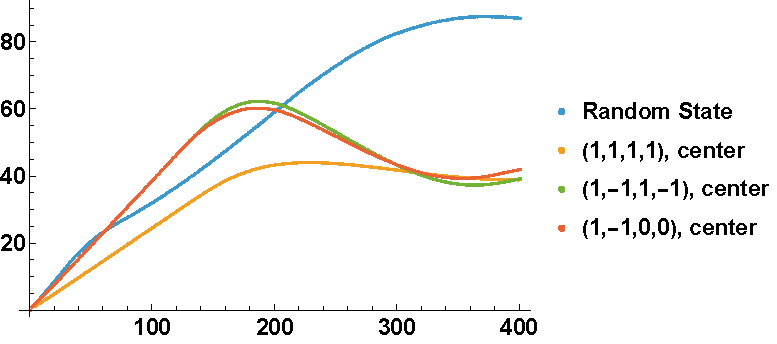
\includegraphics[width=\textwidth]{stdRectComp4.pdf}
\caption{}
\label{fig:der6}
\end{subfigure}

\begin{subfigure}[b]{0.5\textwidth}
\centering
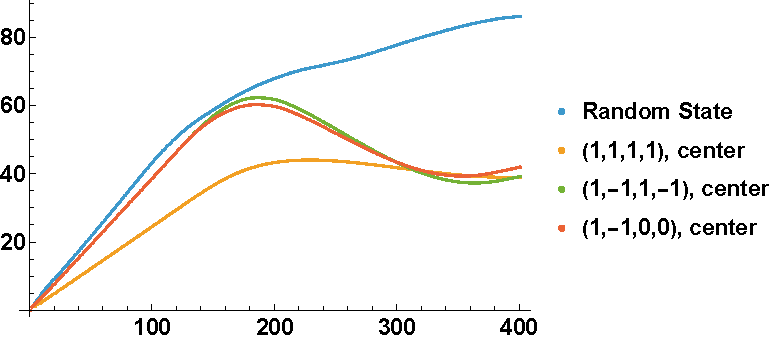
\includegraphics[width=\textwidth]{stdRectComp5.pdf}
\caption{}
\label{fig:izq7}
\end{subfigure}
\caption{Comparación de distintos estados iniciales, empleando un estadio rectangular de dimensiones $L_x=200 \, , L_y=150$.}
\label{fig:ambas5}
\end{figure}
Es notable que el estadio de moneda tiene influencia en que tan 'rápido' se mueve el caminante,
el estado inicial de moneda $(1,1,1,1)$ es el más lento respecto a todos los otros estados evaluados, sin embargo no es concluyente que 
sea el más lento de todos los posibles estados de moneda. Así mismo, los estados iniciales $(1,-1,0,0)\, , (1,-1,1,-1)$ tienen la misma pendiente, por lo menos para el intervalo $[0,140]$.

Empleando como estados inicales de moneda los eigenvectores del operador de Grover (usando $\frac{\pi}{4}$), se obtiene:
\begin{figure}[H]
    \centering
     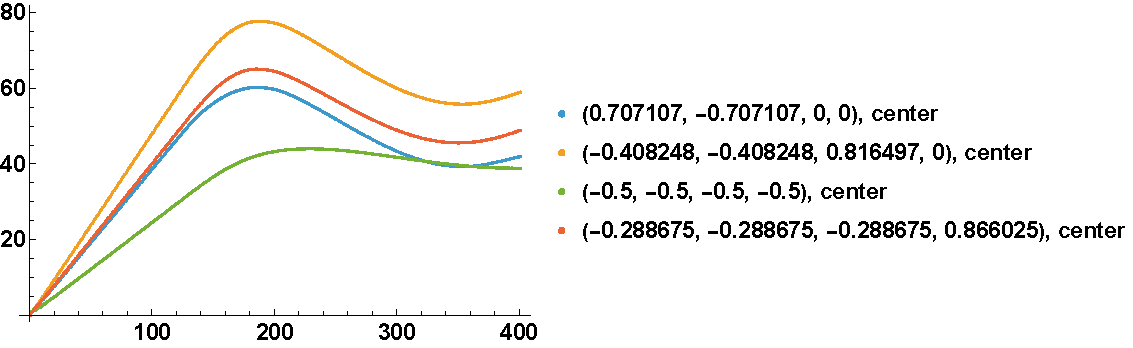
\includegraphics[width=1\textwidth]{stdEigenVecsRect.pdf}
    \caption{Comparación de distintos estados iniciales de moneda que son eigenvectores del operador de Grover, empleando un estadio rectangular de dimensiones $L_x=200 \, , L_y=150$.}
\end{figure}
Es notable que el estado inicial de moneda $(1,1,1,1)$ que se ha estado discutiendo de momento, es eigenvector del operador de Grover.

Una pregunta que vale la pena responder es, dado un estado inicial de moneda, ¿ Qué tanto se diferencia $\sigma$ si el estado localizado empieza en el centro del estadio a si empieza en una posición aleatoria?
\begin{figure}[H]
    \centering
     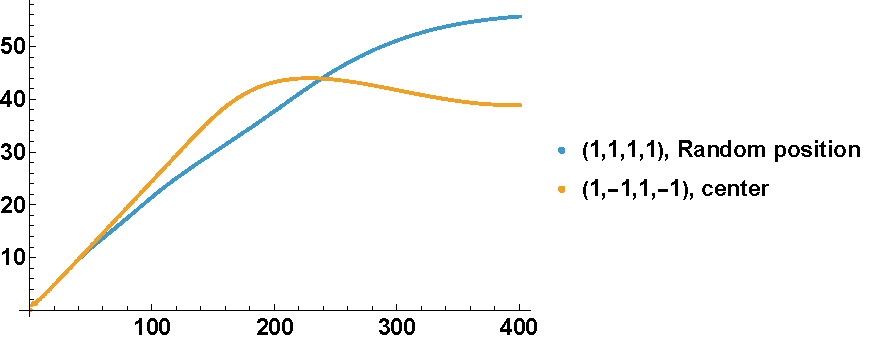
\includegraphics[width=1\textwidth]{stdSameCoinDifPosRect.pdf}
    \caption{Comparación de un mismo estado inicial de moneda para un estado inicial localizado con distinta posición inicial, empleando un estadio rectangular de dimensiones $L_x=200 \, , L_y=150$.}
\end{figure}
Se ve que, por lo menos para un intervalo dado, ambos estados tienen la misma pendiente, pero es claro que para tiempos largos, existen discrepancias.

¿ Será que el estadio Bunimovich induce a un caminata con mayor 'velocidad' que un estadio rectangular?
Emplenado estadios cuya área sea casi la misma (que el grid tenga casi la misma cantidad de puntos), usando un estado inicial de monedad aleatorio (el mismo para ambos), y considerando una posición inicial para ambos estados que estuviese en el centro del estadio, se obtuvo:
\begin{figure}[H]
    \centering
     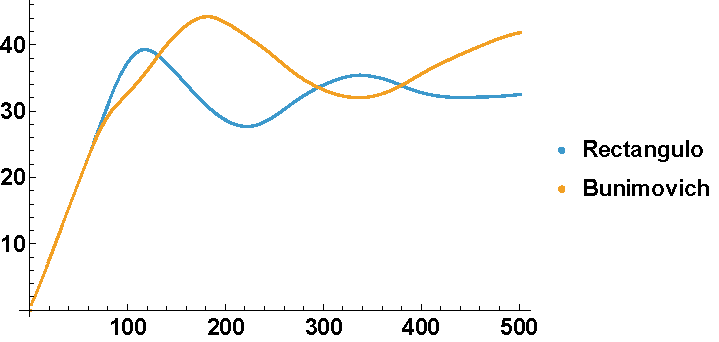
\includegraphics[width=0.7\textwidth]{stdRectvsBun.pdf}
    \caption{Comparación de un mismo estado inicial de moneda para un estado inicial localizado  empleando un estadio rectangular de dimensiones $L_x=120 \, , L_y=110$ y un estadio bunimovich de dimensiones $L= 100 \, , R= 80 $.}
\end{figure}
\end{document}